\documentclass[11pt, oneside]{article} 
\usepackage{geometry}
\geometry{letterpaper} 
\usepackage{graphicx}
	
\usepackage{amssymb}
\usepackage{amsmath}
\usepackage{parskip}
\usepackage{color}
\usepackage{hyperref}

\graphicspath{{/Users/telliott/Github/calculus_book/png/}}
% \begin{center} 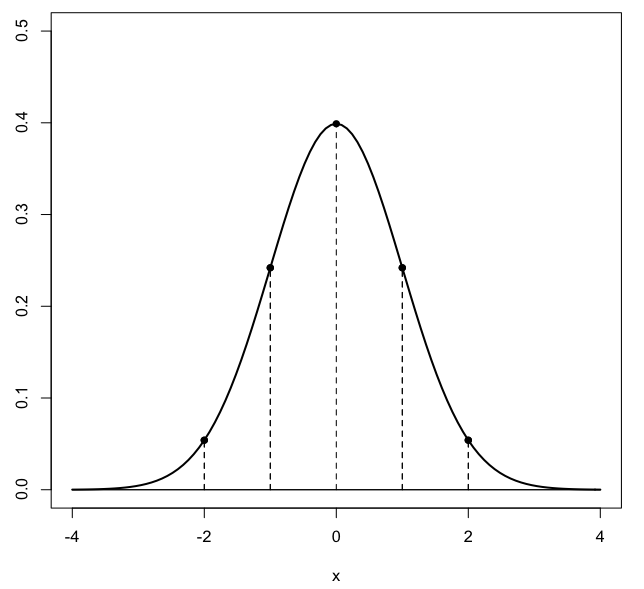
\includegraphics [scale=0.4] {gauss3.png} \end{center}

\title{Arcs of a circle}
\date{}

\begin{document}
\maketitle
\Large
\label{sec:generalized_arc}

Having established some basic facts about circles we can do a bit more.  We will use some of these results later on.

One is to generalize the result for all arcs. The examples so far contain the diameter in some way. Consider the arc swept out by the angle $\theta$ in this figure.
\begin{center} 
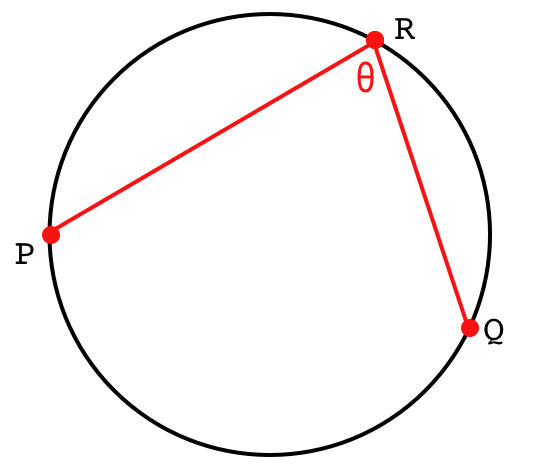
\includegraphics [scale=0.25] {arcs5.png} 
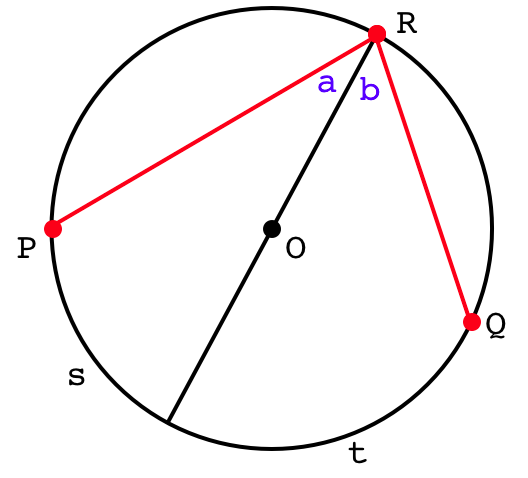
\includegraphics [scale=0.25] {arcs6.png}
\end{center}
We can prove that the measure of the angle $\theta$ is equal to the 1/2 the arc swept out between P and Q. For a simple proof, draw the diameter:
By our previous work:

\[ b = \frac{t}{2} \]
\[ a = \frac{s}{2} \]
\[ \theta = a + b = \frac{s+t}{2} \]

We have proved the theorem for two cases:  where the diameter is one line segment flanking the angle, and where the angle includes the diameter.  However, the theorem is true even if the angle does not include the diameter.
\begin{center} 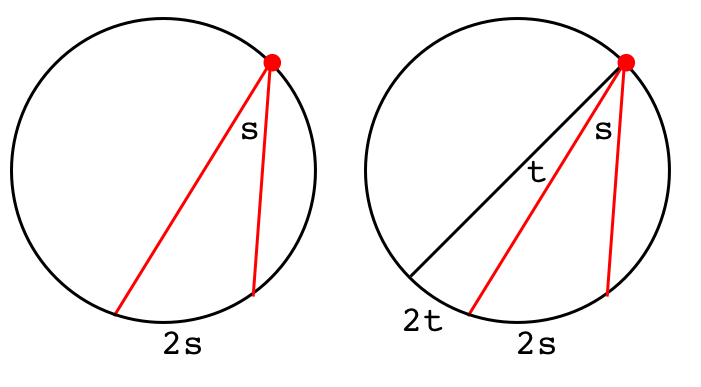
\includegraphics [scale=0.30] {arcs17.png} \end{center}
On the right, draw the diameter.  Notice that we have two arcs which include the diameter:  one with angle $t$ and one with angle $s+t$.  We obtain the generalized arc with angle $s$ by subtraction.

As a corollary, any two angles with vertexes on the circle that cut off the same arc are equal.  In the figure, $s = t$.  Also the triangles are similar triangles.
\begin{center} 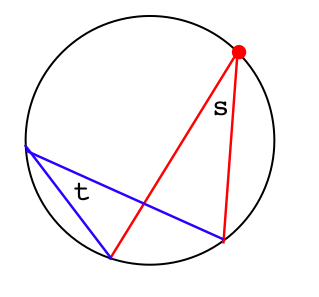
\includegraphics [scale=0.4] {arcs18.png} \end{center}

\subsection*{Intersecting chords}
Given two chords,
to prove:

\[ \theta = 1/2 (s + t) \]

\begin{center} 
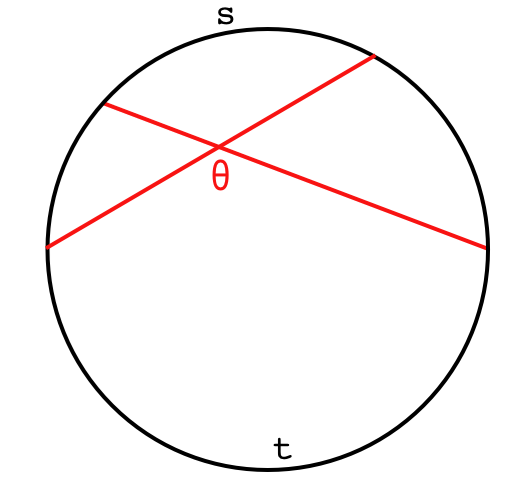
\includegraphics [scale=0.25] {arcs7.png} 
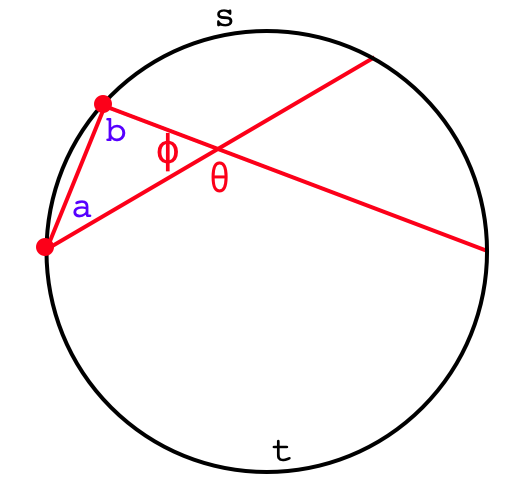
\includegraphics [scale=0.25] {arcs8.png}
\end{center}

$\theta$ is the average of the two arc lengths.
Solution:
Draw a triangle.

\[ a = \frac{s}{2} \]
\[ b = \frac{t}{2} \]
\[ a + b = \theta = \frac{s+t}{2} \]

\subsection*{Tangent and secant}

Rather than having all three points on the circle, one is now outside. We have the same arc swept out by the endpoints ($t$), but the included angle is now smaller, and there is a new small piece of arc length $s$.

\begin{center} 
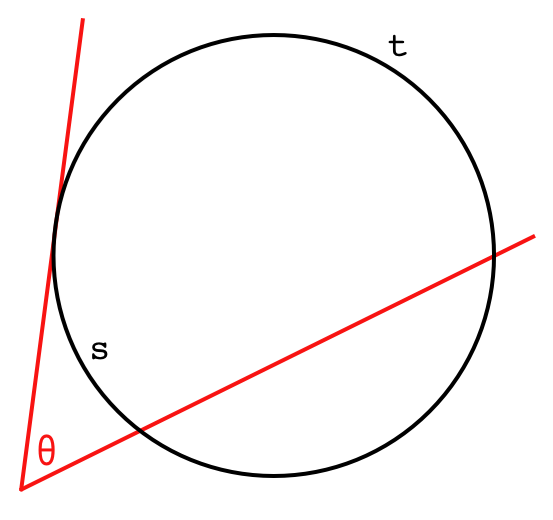
\includegraphics [scale=0.25] {arcs9.png} 
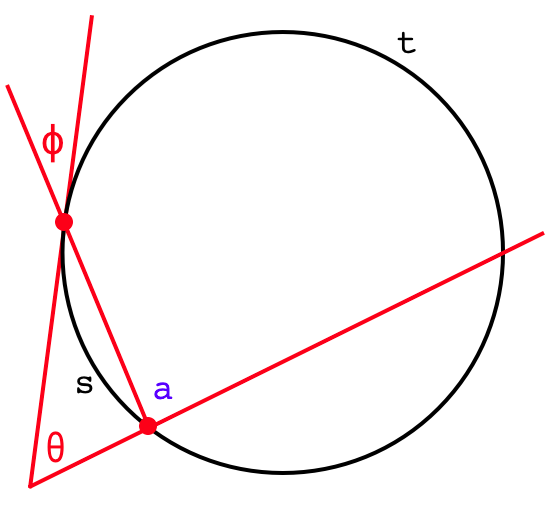
\includegraphics [scale=0.25] {arcs10.png}
\end{center}

To prove:

\[ \theta = \frac{t-s}{2} \]

Solution:
Draw the triangle.
By our previous work (and supplementary angles):

\[ \phi = \frac{s}{2} \]
\[ a = \frac{t}{2} \]

by supplementary angles:

\[ \theta + \phi = a \]
\[ \theta = \frac{t}{2} - \frac{s}{2} \]
\[ = \frac{t-s}{2} \]

\subsection*{Chord segments}

Finally, there is a simple algebraic relationship between chord segments. Draw two chords of the circle and label the lengths of the segments as shown (note: $s$ and $t$ do not refer to arcs any more).

\begin{center} 
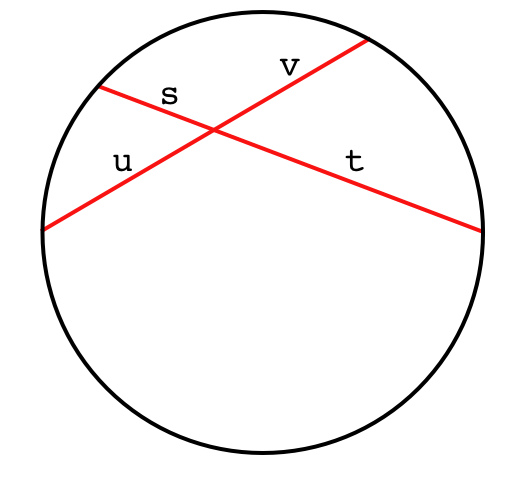
\includegraphics [scale=0.25] {arcs15.png} 
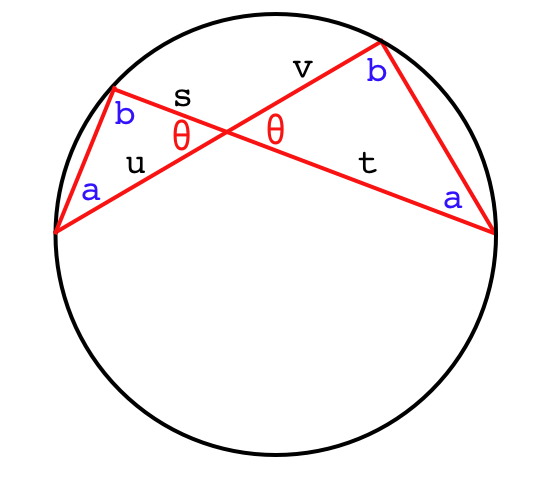
\includegraphics [scale=0.25] {arcs16.png}
\end{center}
Draw the two triangles.
Notice that the two angles labeled $a$ are equal because they sweep out the same arc of the circle, and similarly for the two angles labeled $b$. By similar triangles:

\[ s/u = v/t \]
\[ st = uv \]


\end{document}